\documentclass[10pt]{article}
\usepackage[utf8]{inputenc}
\usepackage[T1]{fontenc}
\usepackage{lmodern}
\usepackage[margin=0.85in,columnsep=0.32in]{geometry}
\usepackage{tikz}
\usetikzlibrary{arrows.meta,positioning,shapes.geometric}
\usepackage{subcaption}
\usepackage{xcolor}
\usepackage[hidelinks]{hyperref}

\setlength{\parindent}{0pt}
\setlength{\parskip}{0.55em}

\definecolor{boxgreen}{RGB}{224,242,224}
\definecolor{boxyellow}{RGB}{252,244,214}
\definecolor{boxred}{RGB}{250,222,222}
\definecolor{boxgray}{RGB}{238,238,235}
\definecolor{lineblack}{RGB}{20,20,20}
\definecolor{barsolid}{RGB}{25,25,25}
\definecolor{bargray}{RGB}{143,143,137}

\title{\LARGE\bfseries When the Agent Decides:\\[2pt] Ten Design Failures in Autonomous Offensive Security Agents}
\author{
  {\large Ricardo Martínez}\\[2pt]
  {\small Cloud Security \& Applied AI}
}
\date{\small September 2026}

\begin{document}
\twocolumn[
  \begin{@twocolumnfalse}
    \maketitle
    \begin{abstract}
    \noindent
    Autonomous AI agents for penetration testing promise to scale offensive work without scaling the human team. This piece documents ten field observations, drawn from operating one such system against real targets over several months, on why the reliability of these agents depends less on the capability of the model orchestrating them and more on concrete engineering decisions: what the LLM is allowed to decide, where the recall problem actually lives, when a failure is worth retrying, how a finding gets verified (and how the verifier itself gets verified) before it is believed, and how silently a system degrades when its environment, its liveness clock, or its redaction layers fail without making any noise. Ten figures and one comparison table grounded in real measurements are presented, closing with nine design principles applicable to any agentic system operating against real attack surface.
    \end{abstract}
    \vspace{1.2em}
  \end{@twocolumnfalse}
]

\section{The Mirage of Total Autonomy}

The first instinct when building a pentesting agent is to let the language model decide which tool to use at each step. It is also the first source of a coverage problem that stays invisible until someone actually measures it.

In a system with roughly sixty available attack capabilities (injection, SSRF, deserialization, secret leakage, access control, JWT, GraphQL), auditing how many ran with guaranteed certainty on every run produced an uncomfortable number: fewer than twenty. Everything else only ran if the agent, in that moment, decided it was worth calling. One concrete test confirmed it: a domain reconnaissance technique showed up in one run and vanished in the next against the exact same target, with nothing in the environment having changed.

\begin{figure}[h]
\centering
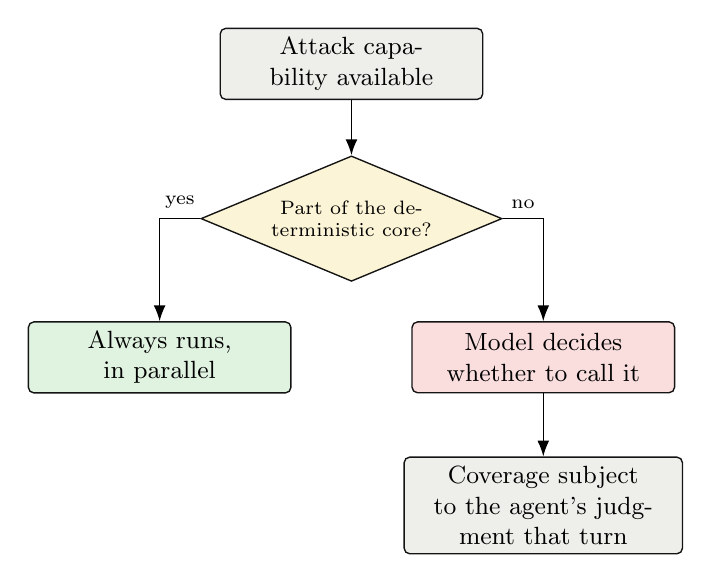
\begin{tikzpicture}[
  node distance=7mm and 8mm,
  box/.style={rectangle, rounded corners=2pt, draw=lineblack, text width=3.1cm, align=center, font=\small, minimum height=9mm, line width=0.5pt},
  dec/.style={diamond, draw=lineblack, aspect=2.4, text width=2.5cm, align=center, font=\scriptsize, inner sep=1pt, line width=0.5pt},
  arr/.style={-{Latex[length=2mm]}, line width=0.5pt}
]
\node[box, fill=boxgray] (cap) {Attack capability available};
\node[dec, fill=boxyellow, below=of cap] (dec1) {Part of the deterministic core?};
\node[box, fill=boxgreen, below left=9mm and -2mm of dec1] (yes) {Always runs, in parallel};
\node[box, fill=boxred, below right=9mm and -2mm of dec1] (no) {Model decides whether to call it};
\node[box, fill=boxgray, below=8mm of no, text width=3.3cm] (out) {Coverage subject to the agent's judgment that turn};

\draw[arr] (cap) -- (dec1);
\draw[arr] (dec1.west) -| node[above,pos=0.25,font=\scriptsize]{yes} (yes);
\draw[arr] (dec1.east) -| node[above,pos=0.25,font=\scriptsize]{no} (no);
\draw[arr] (no) -- (out);
\end{tikzpicture}
\caption{Coverage arbitration. Of \textasciitilde60 available attack capabilities, fewer than 20 ran with guaranteed certainty on every run; the rest were subject to the agent's judgment call each turn.}
\label{fig:coverage}
\end{figure}

The engineering answer was not to tune the prompt so the agent would ``remember'' to use more tools (Figure~\ref{fig:coverage}). It was to pull high-value, low-false-positive-risk capabilities out of the LLM's discretionary territory entirely and turn them into a deterministic sweep that always runs, in parallel, before the agent even enters the picture. The model is left for what genuinely requires judgment: chaining findings together, prioritizing ambiguous surface area, writing up context.

Taken to its final form, the complete pipeline of a real engagement looks like Figure~\ref{fig:pipeline}: a long chain of deterministic steps that always run, with a single discretionary hinge in the middle.

\begin{figure*}[t]
\centering
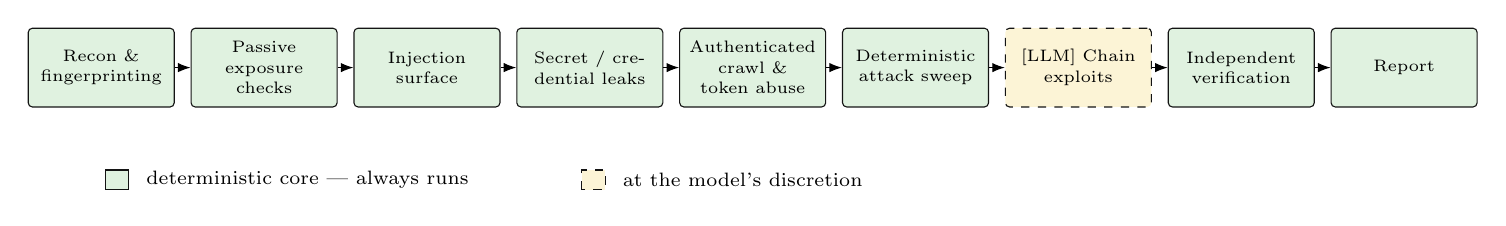
\begin{tikzpicture}[
  node distance=2mm,
  chip/.style={rectangle, draw=lineblack, rounded corners=1.5pt, minimum height=10mm, text width=1.62cm, align=center, font=\fontsize{6.3}{7.4}\selectfont, line width=0.4pt},
  arr/.style={-{Latex[length=1.6mm]}, line width=0.4pt}
]
\node[chip, fill=boxgreen] (c1) {Recon \& fingerprinting};
\node[chip, fill=boxgreen, right=of c1] (c2) {Passive exposure checks};
\node[chip, fill=boxgreen, right=of c2] (c3) {Injection surface};
\node[chip, fill=boxgreen, right=of c3] (c4) {Secret / credential leaks};
\node[chip, fill=boxgreen, right=of c4] (c5) {Authenticated crawl \& token abuse};
\node[chip, fill=boxgreen, right=of c5] (c6) {Deterministic attack sweep};
\node[chip, fill=boxyellow, right=of c6, dashed] (c7) {[LLM] Chain exploits};
\node[chip, fill=boxgreen, right=of c7] (c8) {Independent verification};
\node[chip, fill=boxgreen, right=of c8] (c9) {Report};

\foreach \a/\b in {c1/c2,c2/c3,c3/c4,c4/c5,c5/c6,c6/c7,c7/c8,c8/c9}
  \draw[arr] (\a) -- (\b);

\draw[fill=boxgreen, draw=lineblack, line width=0.4pt] (0.05,-1.55) rectangle (0.35,-1.3);
\node[right=1mm of {(0.35,-1.425)}, anchor=west, font=\scriptsize] {deterministic core --- always runs};
\draw[fill=boxyellow, draw=lineblack, dashed, line width=0.4pt] (6.1,-1.55) rectangle (6.4,-1.3);
\node[right=1mm of {(6.4,-1.425)}, anchor=west, font=\scriptsize] {at the model's discretion};
\end{tikzpicture}
\caption{The actual shape of an end-to-end pentest pipeline. Of nine representative stages, eight are a deterministic sweep that always runs; only exploit chaining is left to the model's discretion, precisely because deciding \emph{whether} to combine two findings is the kind of judgment worth delegating.}
\label{fig:pipeline}
\end{figure*}

\section{Recall Is a Discovery Problem Before It's a Detection Problem}

When a scanner fails to find a real vulnerability, the instinct is to suspect the detector: the payload was wrong, the confirmation engine was too conservative. In practice, the more common cause sat one step earlier: the detector never saw the vulnerable endpoint, because the surface-discovery stage never put it on the table.

\begin{figure}[h]
\centering
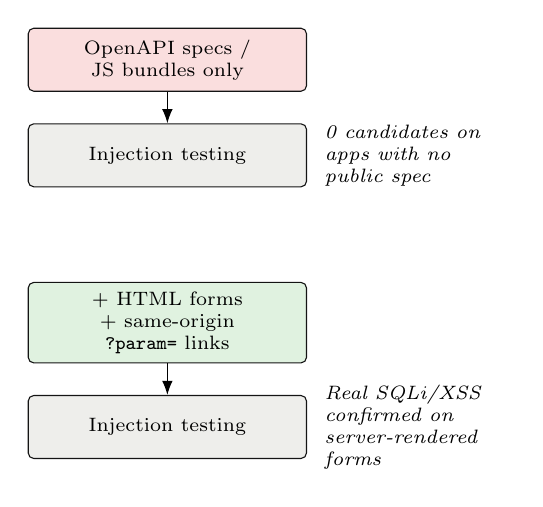
\begin{tikzpicture}[font=\scriptsize]
\node[rectangle, draw=lineblack, fill=boxred, rounded corners=2pt, text width=3.3cm, align=center, minimum height=8mm, line width=0.4pt] (a1) {OpenAPI specs / JS bundles only};
\node[rectangle, draw=lineblack, fill=boxgray, rounded corners=2pt, text width=3.3cm, align=center, minimum height=8mm, line width=0.4pt, below=4mm of a1] (a2) {Injection testing};
\node[font=\scriptsize\itshape, right=1mm of a2, text width=2.1cm] {0 candidates on apps with no public spec};
\draw[-{Latex[length=1.8mm]}, line width=0.4pt] (a1) -- (a2);

\node[rectangle, draw=lineblack, fill=boxgreen, rounded corners=2pt, text width=3.3cm, align=center, minimum height=10mm, line width=0.4pt, below=12mm of a2] (b1) {+ HTML forms \\ + same-origin \texttt{?param=} links};
\node[rectangle, draw=lineblack, fill=boxgray, rounded corners=2pt, text width=3.3cm, align=center, minimum height=8mm, line width=0.4pt, below=4mm of b1] (b2) {Injection testing};
\node[font=\scriptsize\itshape, right=1mm of b2, text width=2.3cm] {Real SQLi/XSS confirmed on server-rendered forms};
\draw[-{Latex[length=1.8mm]}, line width=0.4pt] (b1) -- (b2);
\end{tikzpicture}
\caption{Widening surface discovery, with zero changes to the confirmation engine, moved recall from 0 to real confirmed findings. The test app had no OpenAPI spec at all: its parameters lived only in server-rendered forms.}
\label{fig:discovery}
\end{figure}

Figure~\ref{fig:discovery} documents the case: the exact same injection-confirmation engine, unchanged, went from having nothing to test to confirming real vulnerabilities the moment discovery started parsing forms and same-origin \texttt{?param=} links, on top of the OpenAPI specs and JS bundles it already covered. The detection engine was never the problem. Before tuning payloads or confirmation thresholds, it is worth confirming that the discovered surface actually includes where the vulnerability lives.

\section{Not All Retries Are Equal}

An adversarial code audit found the same fragility pattern repeated across more than thirty distinct call sites: a single network request, and any exception at all --- a timeout, a connection reset, a transient 5xx --- was treated as a definitive result. A network blip during discovery or confirmation turned into a silent miss, indistinguishable from a genuinely clean target.

\begin{figure}[h]
\centering
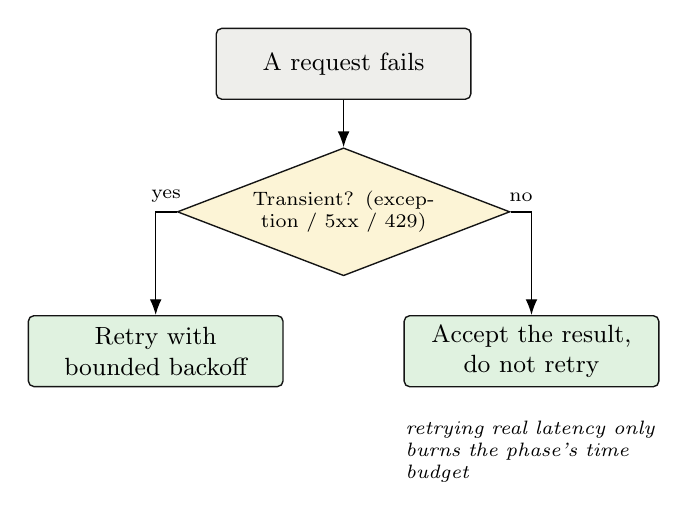
\begin{tikzpicture}[
  node distance=6mm and 7mm,
  box/.style={rectangle, rounded corners=2pt, draw=lineblack, text width=3.0cm, align=center, font=\small, minimum height=9mm, line width=0.5pt},
  dec/.style={diamond, draw=lineblack, aspect=2.6, text width=2.6cm, align=center, font=\scriptsize, inner sep=1pt, line width=0.5pt},
  arr/.style={-{Latex[length=2mm]}, line width=0.5pt}
]
\node[box, fill=boxgray] (f1) {A request fails};
\node[dec, fill=boxyellow, below=of f1] (d1) {Transient? (exception / 5xx / 429)};
\node[box, fill=boxgreen, below left=9mm and -3mm of d1] (y1) {Retry with bounded backoff};
\node[box, fill=boxgreen, below right=9mm and -3mm of d1] (n1) {Accept the result, do not retry};
\node[font=\scriptsize\itshape, below=3mm of n1, text width=3.2cm] {retrying real latency only burns the phase's time budget};

\draw[arr] (f1) -- (d1);
\draw[arr] (d1.west) -| node[above,pos=0.25,font=\scriptsize]{yes} (y1);
\draw[arr] (d1.east) -| node[above,pos=0.25,font=\scriptsize]{no} (n1);
\end{tikzpicture}
\caption{Bounded retry only on transient failure. Retrying a genuine timeout against a slow target does not improve recall, and can exhaust the phase's time budget --- indiscriminate retry is as damaging as never retrying at all.}
\label{fig:retry}
\end{figure}

The fix (Figure~\ref{fig:retry}) was not to retry everything, but to distinguish the type of failure: only a connection exception, a 5xx, or a 429 (rate limit) triggers a bounded retry with backoff; a definitive response --- including a genuine timeout against a slow target --- is accepted and never retried. An additional nuance surfaced while debugging a genuinely unstable test target under load: the exact same code passed and failed across different runs against the same target, with nothing changed in between. The lesson there was to separate two distinct questions before ``fixing'' anything: did the code regress, or is the test target simply unstable? Confusing the two leads to chasing bugs that do not exist.

\section{Adversarial Verification, Not Optional}

An agent that reports its own findings with no one else questioning them has a structural conflict of interest: it was trained to complete the task, not to doubt itself.

\begin{figure}[h]
\centering
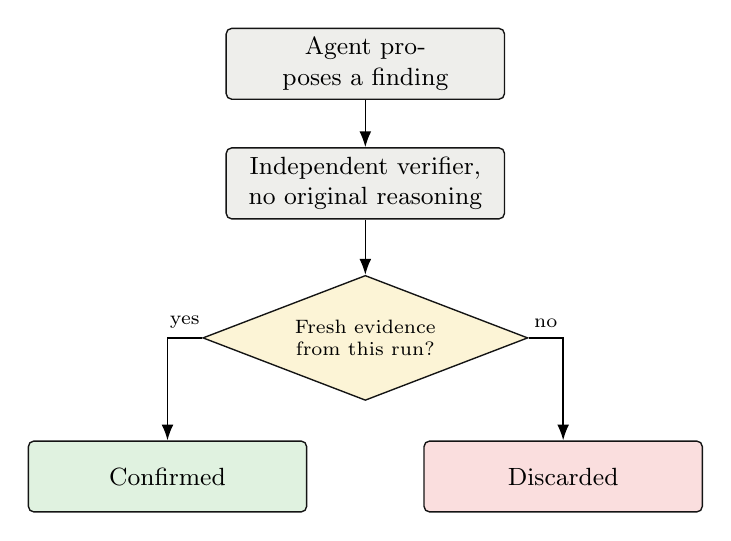
\begin{tikzpicture}[
  node distance=6mm and 8mm,
  box/.style={rectangle, rounded corners=2pt, draw=lineblack, text width=3.3cm, align=center, font=\small, minimum height=9mm, line width=0.5pt},
  dec/.style={diamond, draw=lineblack, aspect=2.6, text width=2.7cm, align=center, font=\scriptsize, inner sep=1pt, line width=0.5pt},
  arr/.style={-{Latex[length=2mm]}, line width=0.5pt}
]
\node[box, fill=boxgray] (a1) {Agent proposes a finding};
\node[box, fill=boxgray, below=of a1] (a2) {Independent verifier, no original reasoning};
\node[dec, fill=boxyellow, below=7mm of a2] (a3) {Fresh evidence from this run?};
\node[box, fill=boxgreen, below left=9mm and -3mm of a3] (a4) {Confirmed};
\node[box, fill=boxred, below right=9mm and -3mm of a3] (a5) {Discarded};

\draw[arr] (a1) -- (a2);
\draw[arr] (a2) -- (a3);
\draw[arr] (a3.west) -| node[above,pos=0.25,font=\scriptsize]{yes} (a4);
\draw[arr] (a3.east) -| node[above,pos=0.25,font=\scriptsize]{no} (a5);
\end{tikzpicture}
\caption{Verification pipeline. The verification step runs on a separate model instance, without the reasoning thread that produced the original finding.}
\label{fig:verify}
\end{figure}

In one run against a production target, the attack agent reported 7 critical or high severity findings in a single pass. The pipeline in Figure~\ref{fig:verify}, run immediately after, discarded 6 of the 7 for lack of fresh evidence. The cause, found by reading the agent's exact prompt: an instruction told it ``don't re-test what's already confirmed from previous runs.'' The agent cited historical findings as if they belonged to this run, without executing a single new tool against them.

The instruction was not wrong by carelessness, it was wrong because it optimized for the wrong thing: saving time by skipping re-confirmation of the obvious, without accounting for the fact that a language model does not distinguish between ``this is already known'' and ``I can claim this as my own.'' The fix was not to ban historical context, but to change its function: from fact to hint.

The system, in this case, worked exactly as it should. The verification layer caught 86\% of the noise. But a system that needs that layer to avoid lying by accident deserves the same structural distrust applied to any unverified source, even when it arrives dressed as a technical report.

\section{Verifying the Verifier}

The verification layer from the previous section solves one problem and creates a subtler new one: who audits whether the verifier itself keeps measuring something real? A concrete case exposed this. A test harness checked that every mandatory pipeline phase had run, comparing against a reference list maintained by hand inside the harness itself. As the real pipeline gained and lost phases across successive iterations, that reference list was not updated at the same pace. The result: the check kept reporting success, always, regardless of what actually ran --- a tautological test that had stopped testing anything.

\begin{figure}[h]
\centering
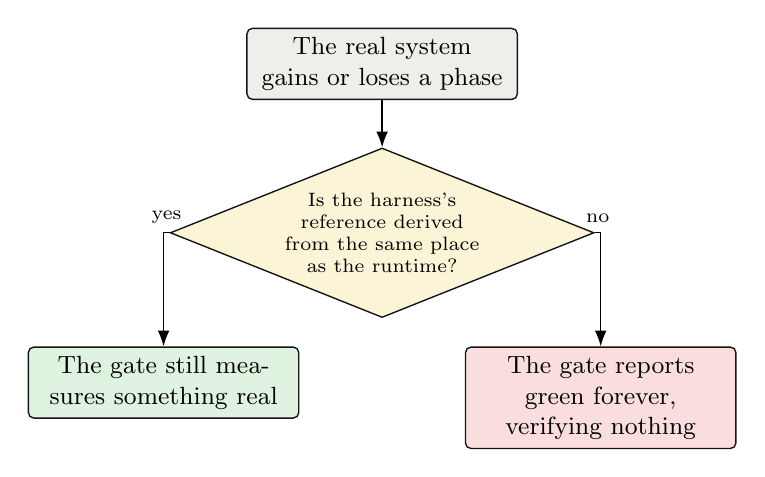
\begin{tikzpicture}[
  node distance=6mm and 8mm,
  box/.style={rectangle, rounded corners=2pt, draw=lineblack, text width=3.2cm, align=center, font=\small, minimum height=9mm, line width=0.5pt},
  dec/.style={diamond, draw=lineblack, aspect=2.5, text width=2.6cm, align=center, font=\scriptsize, inner sep=1pt, line width=0.5pt},
  arr/.style={-{Latex[length=2mm]}, line width=0.5pt}
]
\node[box, fill=boxgray] (v1) {The real system gains or loses a phase};
\node[dec, fill=boxyellow, below=of v1] (v2) {Is the harness's reference derived from the same place as the runtime?};
\node[box, fill=boxgreen, below left=9mm and -3mm of v2] (v3) {The gate still measures something real};
\node[box, fill=boxred, below right=9mm and -3mm of v2] (v4) {The gate reports green forever, verifying nothing};

\draw[arr] (v1) -- (v2);
\draw[arr] (v2.west) -| node[above,pos=0.25,font=\scriptsize]{yes} (v3);
\draw[arr] (v2.east) -| node[above,pos=0.25,font=\scriptsize]{no} (v4);
\end{tikzpicture}
\caption{A verifier with its own hand-maintained copy of the truth, not derived from the same source as the real system, drifts silently. The gate never fails again --- not because the system is perfect, but because the gate stopped comparing against anything real.}
\label{fig:metaverify}
\end{figure}

The fix (Figure~\ref{fig:metaverify}) was to make the reference list derive from the same place the runtime pulls its phases from, instead of living as a hand-maintained parallel copy. Any verification layer --- this section's or the previous one's --- is itself code that can rot silently if its own notion of ``truth'' isn't tied to the same source as the system it watches.

\section{An Evidence Hierarchy}

Not every ``confirmed finding'' a security AI agent produces carries the same evidentiary weight. Ranking confirmation techniques by how hard they are to false-positive changes entirely how an AI-generated security report should be read.

\begin{figure}[h]
\centering
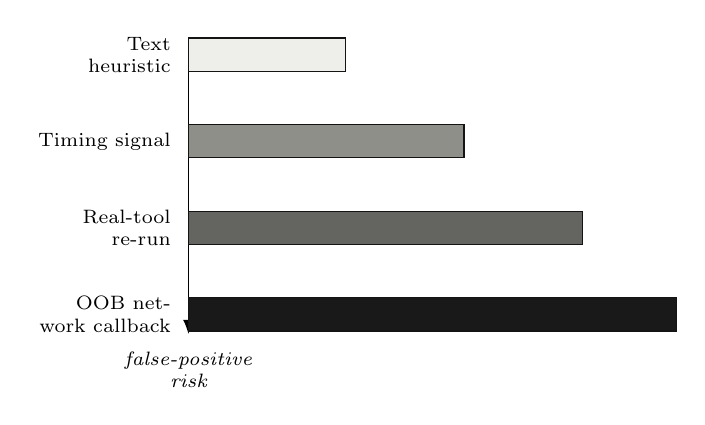
\begin{tikzpicture}[font=\scriptsize]
\draw[-{Latex[length=1.8mm]}, line width=0.5pt] (0,0.1) -- (0,-3.55) node[below, font=\scriptsize\itshape, text width=2.4cm, align=center, yshift=-1mm]{false-positive\\risk};

\node[anchor=east, text width=1.7cm, align=right] at (-0.1,0) {Text heuristic};
\draw[draw=lineblack,fill=boxgray,line width=0.4pt] (0,-0.21) rectangle (2.0,0.21);

\node[anchor=east, text width=1.7cm, align=right] at (-0.1,-1.1) {Timing signal};
\draw[draw=lineblack,fill=bargray,line width=0.4pt] (0,-1.31) rectangle (3.5,-0.89);

\node[anchor=east, text width=1.7cm, align=right] at (-0.1,-2.2) {Real-tool re-run};
\draw[draw=lineblack,fill=bargray!70!black,line width=0.4pt] (0,-2.41) rectangle (5.0,-1.99);

\node[anchor=east, text width=1.7cm, align=right] at (-0.1,-3.3) {OOB network callback};
\draw[draw=lineblack,fill=barsolid,line width=0.4pt] (0,-3.51) rectangle (6.2,-3.09);
\end{tikzpicture}
\caption{Confidence hierarchy for automated confirmation techniques. The out-of-band network callback, where the target itself makes an outbound request to a unique domain generated for that specific probe, is self-contained proof: it requires no interpretation from the model at all.}
\label{fig:hierarchy}
\end{figure}

When a system has an out-of-band network callback technique available (Figure~\ref{fig:hierarchy}), the correct design decision is to run it every time the scan mode allows, not to leave it as one option among dozens the agent may or may not choose to call.

\section{The Model Isn't the Bottleneck}

The natural assumption is that a bigger, more specialized, or ``uncensored'' model produces better offensive security results. Put to a controlled test, that assumption did not hold.

The lesson is not that specialized models are bad. It is that reliably orchestrating tools within a structured contract is a distinct skill from ``knowing offensive security.'' Four local models were benchmarked under the exact same tool-calling contract used by the orchestrator; results are summarized in Table~\ref{tab:models}.

\begin{table*}[t]
\centering
\small
\begin{tabular}{|p{2.9cm}|p{1.0cm}|p{3.4cm}|p{2.4cm}|p{2.4cm}|}
\hline
\textbf{Model} & \textbf{Params} & \textbf{Tool-calling contract} & \textbf{Recall / usability} & \textbf{Runtime / verdict} \\
\hline
Base & 9B & Honored without exception & 6/6 known vulnerabilities & 21.5 min --- reference \\
\hline
``Uncensored'' fine-tune & 9B & Honored without exception & 6/6 known vulnerabilities & 60.4 min (2.8\texttimes) + 1 new FP from mistaking a broken tool install for a real finding \\
\hline
Offensive-specialized A & 7B & Ollama reports it as tool-capable, but it fabricates its own XML instead of filling \texttt{tool\_calls} & Unusable as an agent & Complex prompt: 33+ min, never closed the task \\
\hline
Offensive-specialized B & 8B & Rejected outright (completion-only architecture, no tool support) & Unusable as an agent & 4.9s in pure Q\&A mode --- correctly cited the CVE queried, but never executes a tool \\
\hline
\end{tabular}
\caption{Empirical comparison of four local models under the orchestrator's exact tool-calling contract. The two ``offensive-specialized'' models fail before recall can even be measured: one invents its own output format, the other doesn't declare tool support at all. Both are useful as security Q\&A or synthesis models; neither works as an agent.}
\label{tab:models}
\end{table*}

Neither offensive-specialized model made it as far as measuring recall: one invented its own output syntax instead of using the structured function calls the system expected; the other rejected the request at the architecture level, since its model family does not implement tool-calling at all. Both proved useful as free-text security Q\&A or synthesis models, but neither could participate in the agentic loop.

\begin{figure*}[t]
\centering
\begin{subfigure}[b]{0.47\textwidth}
\centering
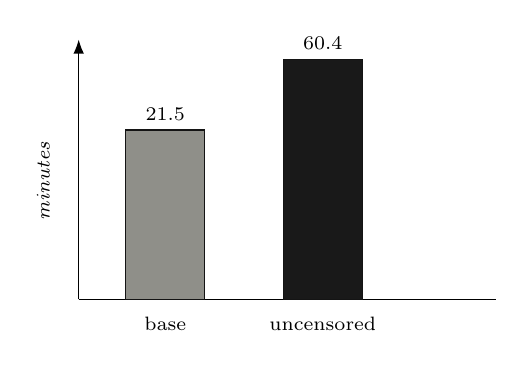
\begin{tikzpicture}[font=\scriptsize]
\draw[-{Latex[length=1.8mm]}, line width=0.5pt] (-0.3,0) -- (-0.3,3.3);
\draw[line width=0.5pt] (-0.3,0) -- (5,0);
\draw[draw=lineblack,fill=bargray,line width=0.4pt] (0.3,0) rectangle (1.3,2.15);
\node[above] at (0.8,2.15) {21.5};
\node[below,yshift=-1mm] at (0.8,0) {base};
\draw[draw=lineblack,fill=barsolid,line width=0.4pt] (2.3,0) rectangle (3.3,3.05);
\node[above] at (2.8,3.05) {60.4};
\node[below,yshift=-1mm] at (2.8,0) {uncensored};
\node[font=\scriptsize\itshape,rotate=90] at (-0.75,1.5) {minutes};
\end{tikzpicture}
\subcaption{Same target, same recall}
\end{subfigure}
\hfill
\begin{subfigure}[b]{0.47\textwidth}
\centering
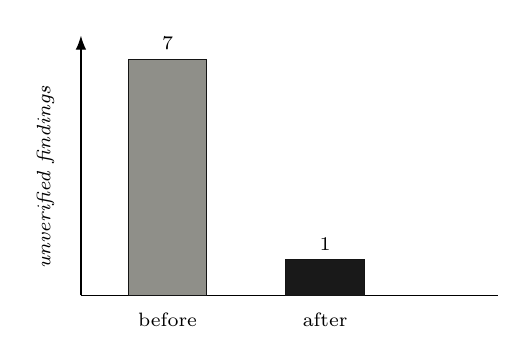
\begin{tikzpicture}[font=\scriptsize]
\draw[-{Latex[length=1.8mm]}, line width=0.5pt] (-0.3,0) -- (-0.3,3.3);
\draw[line width=0.5pt] (-0.3,0) -- (5,0);
\draw[draw=lineblack,fill=bargray,line width=0.4pt] (0.3,0) rectangle (1.3,3.0);
\node[above] at (0.8,3.0) {7};
\node[below,yshift=-1mm] at (0.8,0) {before};
\draw[draw=lineblack,fill=barsolid,line width=0.4pt] (2.3,0) rectangle (3.3,0.45);
\node[above] at (2.8,0.45) {1};
\node[below,yshift=-1mm] at (2.8,0) {after};
\node[font=\scriptsize\itshape,rotate=90] at (-0.75,1.5) {unverified findings};
\end{tikzpicture}
\subcaption{Before / after the prompt fix}
\end{subfigure}
\caption{(a) Two variants of a local \textasciitilde9B-parameter model against the same lab target: identical recall, but the ``uncensored'' variant took 2.8\texttimes\ longer and produced one additional false positive. (b) In the same system, fixing a single prompt instruction reduced from 7 to 1 the critical/high findings reaching verification without fresh evidence.}
\label{fig:compare}
\end{figure*}

\section{Environment Fragility as a Silent Failure}

Of all the possible failure modes, the most dangerous is not the model hallucinating. It is a real, correctly-built tool silently failing to run for a reason entirely unrelated to the system's logic, with nobody noticing because the system keeps producing a report that looks perfectly normal.

A deterministic injection engine failed to run for an entire testing session against a real target. The cause was not in its code: the orchestrating process had been started with an environment variable different from the reference environment, and that single difference made the operating system resolve the binary's name to the wrong executable sharing that name. The visible symptom was one generic error line buried among dozens of log entries, easy to mistake for ``the target wasn't vulnerable'' instead of ``the tool never ran.''

This kind of failure drops real coverage below reported coverage, consistently, for as long as the environmental condition persists. The correct response is not to document ``remember to export the right variable''; that offloads the responsibility onto human memory. The correct response is for the system itself to guarantee its own environmental conditions when executing each tool, regardless of how it was launched.

The same silent-failure pattern shows up at the level of an entire engagement, not just a single tool. An active scan sat marked ``running'' for over an hour with nobody noticing: the target was resetting connections under a web application firewall, the phase's loop froze waiting for a response that never came, and the scan's own heartbeat mechanism froze right along with it --- a process that stops breathing cannot report that it stopped breathing.

\begin{figure}[h]
\centering
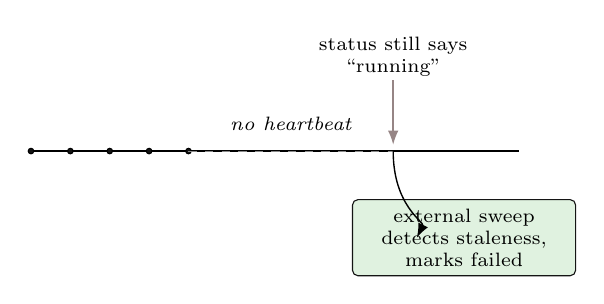
\begin{tikzpicture}[font=\scriptsize]
\draw[line width=0.5pt] (0,0) -- (6.2,0);
\foreach \x in {0,0.5,...,2.0}
  \draw[fill=lineblack] (\x,0) circle (0.035);
\draw[dashed, line width=0.4pt, lineblack!50] (2.0,0) -- (4.6,0);
\node[font=\scriptsize\itshape] at (3.3,0.35) {no heartbeat};
\draw[-{Latex[length=1.8mm]}, line width=0.6pt, boxred!60!black] (4.6,0.9) -- (4.6,0.08);
\node[font=\scriptsize, text width=2.6cm, align=center] at (4.6,1.2) {status still says ``running''};
\node[rectangle, draw=lineblack, fill=boxgreen, rounded corners=2pt, minimum height=8mm, text width=2.6cm, align=center, line width=0.4pt] at (5.5,-1.1) {external sweep detects staleness, marks failed};
\draw[-{Latex[length=1.8mm]}, line width=0.5pt] (4.6,0) .. controls (4.6,-0.7) and (5.0,-0.9) .. (4.9,-1.1);
\end{tikzpicture}
\caption{A process that freezes cannot report that it froze. The task's own heartbeat died along with the task; only an external liveness sweep, unrelated to the loop that failed, could detect and correct the stuck state.}
\label{fig:liveness}
\end{figure}

The lesson in Figure~\ref{fig:liveness} is distinct from the tool with the broken PATH, even though both are silent failures: here, no mechanism \emph{internal} to the task can detect its own freeze, by definition. It takes an external observer --- a periodic sweep, unrelated to the loop being monitored --- that measures liveness by elapsed time, not by the task's own claim that it's still alive.

\section{Defense in Depth for Sensitive Data}

A system investigating real attack surface inevitably touches data that should never reach a report in the clear: credentials, tokens, user listings. The design temptation is to redact that data at the point where it's generated and call it solved. That temptation is exactly the mistake: a single redaction point is, by definition, a single point of failure.

\begin{figure}[h]
\centering
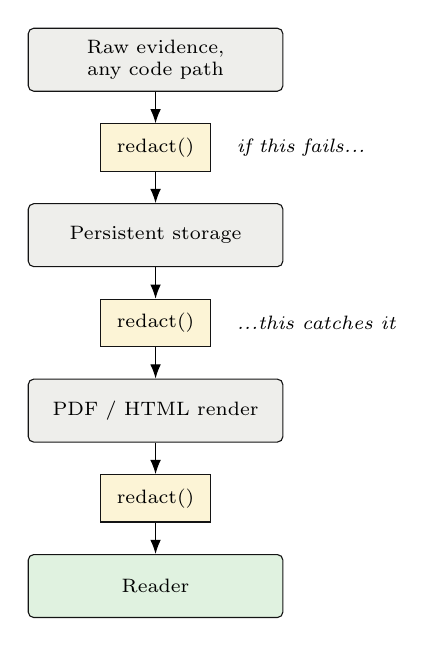
\begin{tikzpicture}[
  node distance=4mm,
  box/.style={rectangle, rounded corners=2pt, draw=lineblack, text width=3.0cm, align=center, font=\scriptsize, minimum height=8mm, line width=0.4pt},
  gate/.style={rectangle, draw=lineblack, fill=boxyellow, minimum height=6mm, minimum width=14mm, font=\scriptsize, line width=0.4pt},
  arr/.style={-{Latex[length=1.8mm]}, line width=0.4pt}
]
\node[box, fill=boxgray] (r1) {Raw evidence, any code path};
\node[gate, below=of r1] (g1) {redact()};
\node[box, fill=boxgray, below=of g1] (r2) {Persistent storage};
\node[gate, below=of r2] (g2) {redact()};
\node[box, fill=boxgray, below=of g2] (r3) {PDF / HTML render};
\node[gate, below=of r3] (g3) {redact()};
\node[box, fill=boxgreen, below=of g3] (r4) {Reader};

\draw[arr] (r1) -- (g1);
\draw[arr] (g1) -- (r2);
\draw[arr] (r2) -- (g2);
\draw[arr] (g2) -- (r3);
\draw[arr] (r3) -- (g3);
\draw[arr] (g3) -- (r4);
\node[font=\scriptsize\itshape, right=2mm of g1, text width=2.1cm] {if this fails...};
\node[font=\scriptsize\itshape, right=2mm of g2, text width=2.1cm] {...this catches it};
\end{tikzpicture}
\caption{Three independent redaction layers, not a sequential trust chain. A new code path that skips the first layer still passes through the other two before reaching a reader.}
\label{fig:redact}
\end{figure}

The real case that forced this design (Figure~\ref{fig:redact}): a new phase of the system generated evidence in a format the first redaction layer didn't know to recognize, and a listing of real usernames slipped through unmasked all the way to the persistence point. It never reached a reader because a second layer, at the persistence point --- which redacts \emph{everything} written, regardless of which phase produced it --- intercepted it there. The property that matters is not that each layer is perfect; it's that no single layer is a requirement for the whole system to be safe.

\section{A One-Time Validation Is Not a Boundary}

Restricting what a scan is allowed to target (never cloud metadata, never private ranges without explicit authorization) sounds, at first glance, like a check performed once, when the request is accepted. That is precisely the surface an attacker --- or a hostile target --- can exploit.

\begin{figure}[h]
\centering
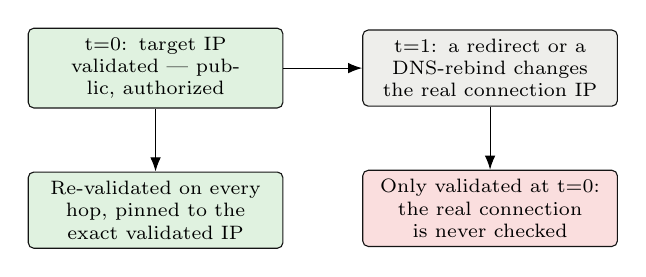
\begin{tikzpicture}[font=\scriptsize]
\node[rectangle, draw=lineblack, fill=boxgreen, rounded corners=2pt, text width=3.0cm, align=center, minimum height=9mm, line width=0.4pt] (t0) {t=0: target IP validated --- public, authorized};
\node[rectangle, draw=lineblack, fill=boxgray, rounded corners=2pt, text width=3.0cm, align=center, minimum height=9mm, line width=0.4pt, right=10mm of t0] (t1) {t=1: a redirect or a DNS-rebind changes the real connection IP};
\draw[-{Latex[length=1.8mm]}, line width=0.4pt] (t0) -- (t1);

\node[rectangle, draw=lineblack, fill=boxred, rounded corners=2pt, text width=3.0cm, align=center, minimum height=9mm, line width=0.4pt, below=8mm of t1] (bad) {Only validated at t=0: the real connection is never checked};
\node[rectangle, draw=lineblack, fill=boxgreen, rounded corners=2pt, text width=3.0cm, align=center, minimum height=9mm, line width=0.4pt, below=8mm of t0] (good) {Re-validated on every hop, pinned to the exact validated IP};
\draw[-{Latex[length=1.8mm]}, line width=0.4pt] (t1) -- (bad);
\draw[-{Latex[length=1.8mm]}, line width=0.4pt] (t0) -- (good);
\end{tikzpicture}
\caption{A front-door validation checks the IP at the moment the request is accepted (t=0); a redirect or a DNS-rebind can change what the system actually connects to afterward (t=1). Closing the window requires re-validating on every hop and pinning the connection to the exact IP that was validated.}
\label{fig:toctou}
\end{figure}

The principle in Figure~\ref{fig:toctou} generalizes beyond network scanning: any security control expressed as ``checked on the way in'' leaves open the window between the check and the actual use. If the system later follows redirects, resolves names again, or reuses a decision made minutes earlier, that window is exploitable. The fix is not a stricter check at the start; it is repeating the same validation at every point where the system actually acts, and tying the action to the exact result of that re-validation.

\section{Design Principles}

\begin{enumerate}
\item \textbf{Critical capabilities are never optional for the model.} If something must always run, make it a deterministic pipeline step, not just another tool among many.
\item \textbf{Recall is won in discovery, not just in detection.} A perfect confirmation engine finds nothing if it's never shown the vulnerable endpoint.
\item \textbf{Retry the transient failure, accept the definitive one.} Retrying every error indiscriminately is as damaging to recall as never retrying at all.
\item \textbf{No finding is trusted in the same pass that produced it.} An independent verification step, without the original reasoning in view, is the difference between a report and a hallucination wearing a report's clothes.
\item \textbf{The verifier needs verifying too.} A test whose own notion of ``truth'' is hand-maintained, not tied to the real source, turns tautological in silence.
\item \textbf{Rank your evidence, and say so in the report.} A network-callback detection and a text-heuristic detection should not reach the reader under the same ``confirmed'' label.
\item \textbf{Historical context is a hint, never a fact.} If a prompt gives the model permission to skip re-verifying something, that something will eventually get reported without evidence.
\item \textbf{The runtime environment is part of the reliability surface.} A system that depends on its environment being configured ``the way it should be'' has a fragile dependency disguised as a technical assumption; this includes being able to detect its own freeze, something no purely internal mechanism can do.
\item \textbf{No security control is a one-time validation.} Repeat the check at every point where the system actually acts, and use independent layers for sensitive data --- never a single point of redaction or validation.
\end{enumerate}

\vspace{0.6em}
{\small\itshape Methodological note: the observations above come from operating a single system in production across several work sessions, not from a controlled study across multiple systems. The figures cited are real measurements from those runs; target, client, and tool names are deliberately omitted for confidentiality.}

\end{document}
